\documentclass[a4paper,11pt]{scrartcl}

\usepackage[utf8]{inputenc}
\usepackage[T1]{fontenc}
\usepackage{amsmath}
\usepackage[left=3cm, right=2cm, top= 2cm, bottom = 2.5cm, includeheadfoot]{geometry}
\usepackage[svgnames]{xcolor}

\usepackage{pdfpages}
\usepackage{listings} 
\lstset{
	basicstyle=\scriptsize\color{Black},
	keywordstyle=\color{SteelBlue}\bfseries,
	language = java,
	numbers=right, numberstyle=\small, stepnumber=5, numbersep=0pt,
	showstringspaces=false}
\usepackage{url}
\usepackage{setspace}
%umgebungen sind \begin(singlespace/onehalfspace/doublespace)
%einfacher eineinhalbfacher und 2facher zeilenabstand
%es kann aber auch nur mit \singlespace \doublespace und \onehalfspacing gearbeitet werden.

\usepackage{times}
\usepackage{graphicx}
\usepackage{color}
\usepackage{fancyhdr}
\pagestyle{fancy}
\lhead{\small Jonas Kordt, Simon Stadlinger}
\chead{\small Serie 5}
\rhead{\small Programmiertechnik II}

\rfoot{}
\cfoot{\thepage}
\lfoot{}

%\pagestyle{headings}

%Befehle um Kopfund Fuszeile Anzupassen:
%\thepage - Seitennummer
%\leftmark - Aktueller Kapitelname "Kapitel X. Name des Kapitels"
%\rightmark - Aktueller Untertitelname "X.X Name des Kapitels
%\chaptername - Das Wort "Kapitel"
%\thechapter - Aktuelle Kapitelnummerierung
%\thesection - Aktuelle Unterkapitelnummerierung
%\slshape - Kursiv und Sanseriv


\begin{document}
\begin{center}
{\LARGE Zusatzaufgabe Code-Coverage}
\end{center}

\section{Umgebung}
Kurzzeitig wurde das build.xml durch diese Zeilen ersetzt
\begin{lstlisting}
<project name="Deque" default="all" basedir=".">
     <property file="build.properties" />
 
     <path id="cobertura.classpath">
          <fileset dir="${cobertura.dir}">
             <include name="cobertura*.jar" />
             <include name="lib/**/*.jar" />
         </fileset>
     </path>
 
     <taskdef classpathref="cobertura.classpath" resource="tasks.properties"/>
 
     <target name="init">
         <mkdir dir="${classes.dir}" />
         <mkdir dir="${instrumented.dir}" />
         <mkdir dir="${reports.xml.dir}" />
         <mkdir dir="${reports.html.dir}" />
          <mkdir dir="${coverage.xml.dir}" />
         <mkdir dir="${coverage.summaryxml.dir}" />
         <mkdir dir="${coverage.html.dir}" />
     </target>
 
     <target name="compile" depends="init">
         <javac srcdir="${src.dir}" destdir="${classes.dir}" debug="yes">
             <classpath refid="cobertura.classpath" />
          </javac>
     </target>
 
     <target name="instrument" depends="init,compile">
         <delete file="cobertura.ser"/>
         <delete dir="${instrumented.dir}" />
 
          <cobertura-instrument todir="${instrumented.dir}">
              
             <ignore regex="org.slf4j.*" />
 
             <fileset dir="${classes.dir}">
                 <include name="**/*.class" />
                 <exclude name="**/*Test.class" />
                 <exclude name="DequePerformance.class" />
             </fileset>
         </cobertura-instrument>
     </target>
     <target name="test" depends="init,compile">
         <junit haltonfailure="yes" fork="yes" dir="${basedir}" failureProperty="test.faile    d">
             <classpath location="${instrumented.dir}" />
             <classpath location="${classes.dir}" />
              <classpath refid="cobertura.classpath" />
 
             <formatter type="xml"/>
             <test name="${testcase}" todir="${reports.xml.dir}" if="testcase" />            
             <batchtest todir="${reports.xml.dir}" unless="testcase">
                 <fileset dir="${src.dir}">
                     <include name="**/*Test.java" />
                     <exclude name="**/DequeTest.java"/>
                 </fileset>
             </batchtest>
         </junit>
 
          <junitreport todir="${reports.xml.dir}">
             <fileset dir="${reports.xml.dir}">
                 <include name="TEST-*.xml" />
             </fileset>
             <report format="frames" todir="${reports.html.dir}" />
         </junitreport>
     </target>
 
     <target name="coverage-check">
         <cobertura-check branchrate="34" totallinerate="100" />
     </target>
 
     <target name="coverage-report">
         <cobertura-report srcdir="${src.dir}" destdir="${coverage.xml.dir}" format="xml" /    >
     </target>
 
     <target name="alternate-coverage-report">
         <cobertura-report destdir="${coverage.html.dir}">
            <fileset dir="${src.dir}">
                <include name="**/*.java"/>
            </fileset>
         </cobertura-report>
     </target>
 
 
     <target name="clean" description="Remove all files created by the build/test process."    >
        <delete dir="${classes.dir}" />
        <delete dir="${instrumented.dir}" />
        <delete dir="${reports.dir}" />
        <delete file="cobertura.log" />
        <delete file="cobertura.ser" />
     </target>
 
     <target name="all" depends="compile,instrument,test,coverage-report, alternate-coverag    e-report"/>
\end{lstlisting} 
und die Datei build.proberties zusätzlich geschrieben
\begin{lstlisting}

 src.dir=src
 
 # The path to cobertura.jar
 cobertura.dir=../cobertura
 
 # Classes generated by the javac compiler are deposited in this directory
 classes.dir=build
 
 # Instrumented classes are deposited into this directory
 instrumented.dir=instrumented
 
 # All reports go into this directory
 reports.dir=reports
 
 # Unit test reports from JUnit are deposited into this directory
 reports.xml.dir=${reports.dir}/junit-xml
 reports.html.dir=${reports.dir}/junit-html
 
 # Coverage reports are deposited into these directories
 coverage.xml.dir=${reports.dir}/cobertura-xml
 coverage.summaryxml.dir=${reports.dir}/cobertura-summary-xml
 coverage.html.dir=${reports.dir}/cobertura-html

\end{lstlisting}


\section{ant all}
Lässt man das build-File ohne spezifizierte Target laufen, wird \texttt{all} ausgeführt. Dabei werden \textbf{drei} neue Ordner angelegt.
\begin{itemize}
\item[\textbf{build}] Die übersetzen Source-Files
\item[\textbf{instrumented}] Die zu traversierenden Class-Files für cubertura
\item[\textbf{report}] Cobertura erstellt hier für die durchlaufenen Tests xml- und html-Zusammenfassungen
\end{itemize}
\begin{center}
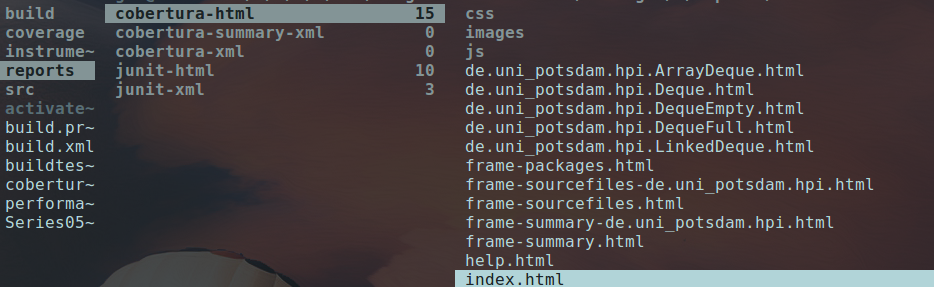
\includegraphics[scale=0.45]{ordner}
\end{center}
Ruft man nun \texttt{index.html} auf, öffnet sich eine Übersicht der getesten Files im Browser von der man sich durch die einzelnen Files manövrieren kann.
\begin{center}
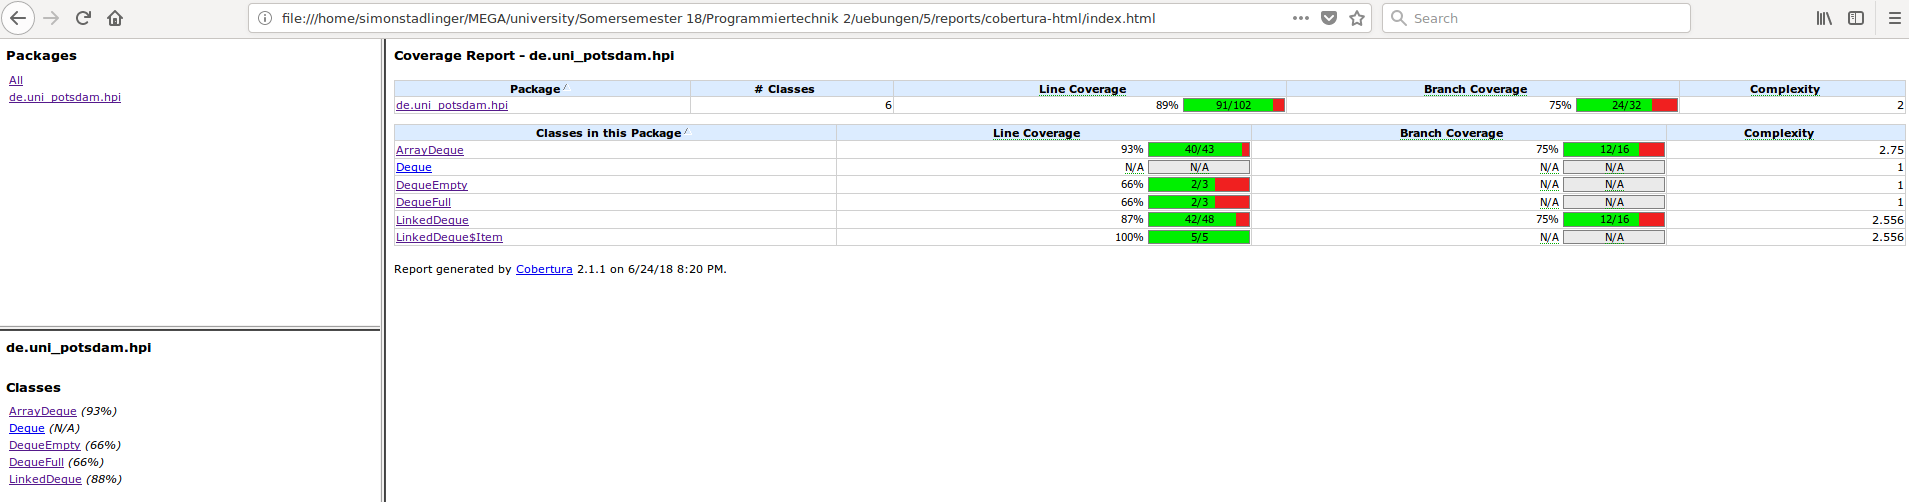
\includegraphics[scale=0.24]{overview}
\end{center}
\newpage
\section{ArrayDequeTest}
\begin{center}
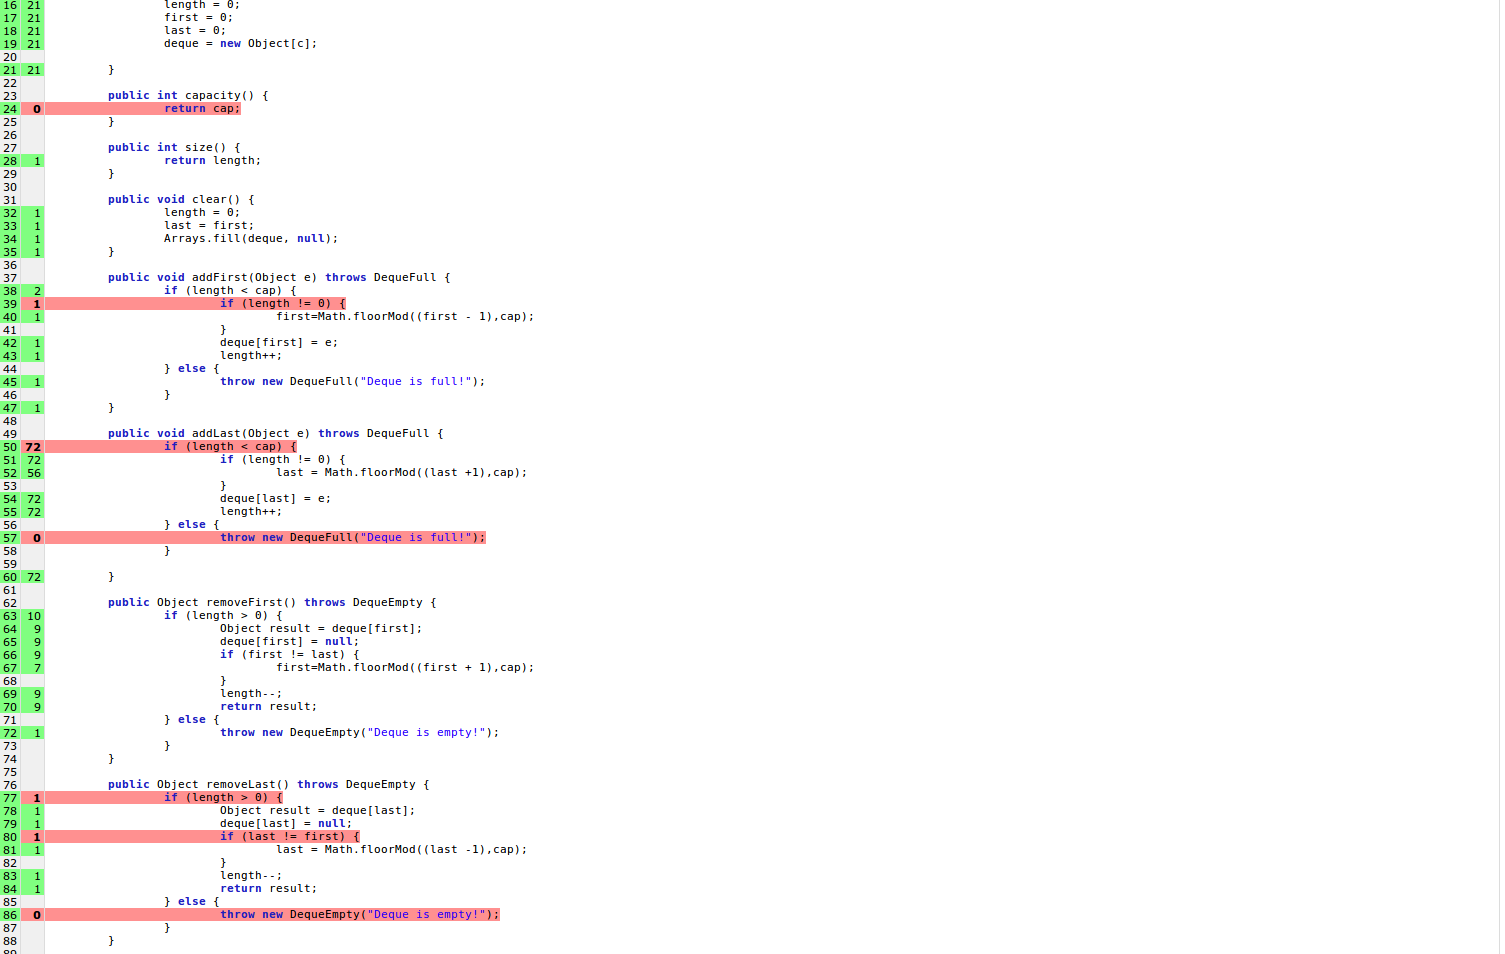
\includegraphics[scale=0.3]{arraydeque}

\end{center}
Der Code von ArrayDeque.java weißt initial eine line-coverage von 93\% auf. Sieht man sich den von cobertura markierten code an, werden drei Zeilen hervorgehoben:
\begin{center}
\begin{lstlisting}
return cap; //in capacity()
...
throw new DequeFull("Deque is full!"); //in addLast()
...
throw new DequeEmpty("Deque is empty!"); //in removeFirst()
\end{lstlisting} 
\end{center}
Für diese Fälle wurde die abstracte Klasse DequeTest um folgendeTests erweitert
\begin{lstlisting}
     @Test 
     public void TestH(){
        //capacity of emptyDeque liefert 10;
        assertEquals("capacity of konstructor and capacity() not equal", (long) 10, emptyDeque.capacity());
    }        
     @Test
     public void TestI() throws Exception{
     //addLast liefert fuer eine volle Deque eine Ausnahme.
      	 try{
       	    fullDeque.addLast(new Object());
       	    fail("addLast() did not throw exception");
      	  }catch (DequeFull e){}
   	 }
    @Test
   	 public void testJ() throws Exception{
     	//removeFirst liefert fuer eine leere Deque eine Ausnahme.
        try{
            emptyDeque.removeFirst();
            fail("removeFirst() did not throw exception");
        }catch (DequeEmpty e){}
     }
 

\end{lstlisting}
Nach dieser Maßnahme ist die Line-Coverage von ArrayDeque auf 100\% gestiegen.
\begin{center}
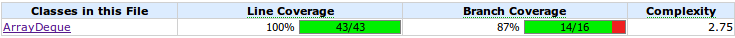
\includegraphics[scale=0.5]{ArrayDeque100}
\end{center}
\section{LinkedDequeTest}
Wie in Abbildung 2 zu sehen, hatte LinkedDeque eine Code-Coverage von 87\%. Da LinkedDequeTest und ArrayDequeTest von DeqeuTest erben, werden die neuen Tests auch für LinkedDeque ausgeführt und erhöhen dessen Line-Coverage auf 93\%.
\begin{center}
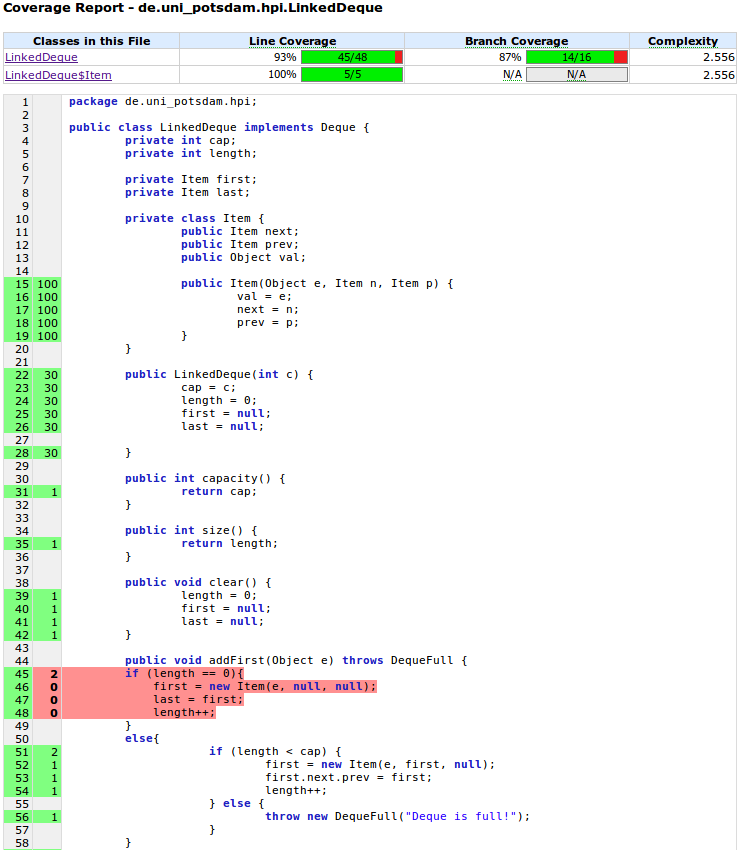
\includegraphics[scale=0.45]{linkeddeque}
\end{center}
Für die nicht abgedeckten Lines
\begin{lstlisting}
if (length == 0){ //in addFirst()
	first = new Item(e, null, null);
	last = first;
	length++;
\end{lstlisting}
wurde folgender Test geschrieben
\begin{lstlisting}
@Test 
public void testK() throws Exception{
    //Groesse von emptyDeque nach einfuegen von einem Element ist 1
	Object e = new Object();
    emptyDeque.addFirst(e);
    assertEquals("emptyDeque after insert length is not 1", (long) 1, emptyDeque.size());
}
\end{lstlisting}
Die Line Coverage von LinkedDeque beträgt nun auch 100\%
\begin{center}
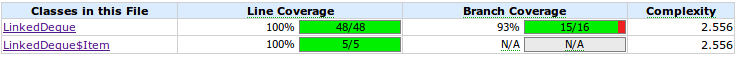
\includegraphics[scale=0.5]{LinkedDeque100}
\end{center}
Um im gesamten Paket Line-Coverage 100\% zu erhalten, mussten die beiden getesten Files an einer Stelle abgewandelt werden. Die Exceptinons wurden jedes mal nur mit einem übergebenen String geworfen. Um die in Abbildung 2 dargestellten 2/3 bei DequeFull und DequeEmpty auf 3/3 zu erhöhen wurden in LinkedDeque bei 2 von 4 Exceptions die Stringparametern aus den Exceptions-Aufrufen entfernt.
\end{document}
